\documentclass[11pt]{article}

\usepackage[letterpaper,margin=1in]{geometry}
\usepackage{lipsum}

% ToC
\usepackage{blindtext} 
\usepackage[linktocpage]{hyperref}
\usepackage{bookmark}
\usepackage[compact]{titlesec}

% bib
%\usepackage[round]{natbib}
\usepackage[square,sort,numbers]{natbib}

% Math Imports
\usepackage{amsmath, amssymb, bm, fancyhdr, sectsty, dsfont, mathtools}

% Tikz
\usepackage{tikz}
\usetikzlibrary{bayesnet}
\usetikzlibrary{arrows}

\usepackage{wrapfig}
\usepackage{comment}
\usepackage{subcaption}
\usepackage{cleveref}

% Symbols
\newcommand\ind{\protect\mathpalette{\protect\independenT}{\perp}}
\def\independenT#1#2{\mathrel{\rlap{$#1#2$}\mkern2mu{#1#2}}}
\newcommand\norm[1]{\left\lVert#1\right\rVert}
\newcommand\set[1]{\left\{#1\right\}}

\newcommand\RNN{\mathrm{RNN}}
\newcommand\MLP{\mathrm{MLP}}
\newcommand\enc{\mathrm{enc}}
\newcommand\softmax{\mathrm{softmax}}

% Distributions
\newcommand{\Cat}{\mathrm{Cat}}
\newcommand\Expo{\mathrm{Expo}}
\newcommand\Bern{\mathrm{Bern}}
\newcommand\Pois{\mathrm{Pois}}
\newcommand\Bin{\mathrm{Bin}}
\newcommand\Unif{\mathrm{Unif}}
\newcommand\Betad{\mathrm{Beta}}
\newcommand\Gammad{\mathrm{Gamma}}
\newcommand\Geom{\mathrm{Geom}}
\newcommand\Logd{\mathrm{Logistic}}

\newcommand\E[1]{\mathbb{E}\left[#1\right]}
\newcommand\Es[2]{\mathbb{E}_{#1}\left[#2\right]}
\newcommand{\Var}{\mathrm{Var}}
\newcommand{\Cov}{\mathrm{Cov}}
\newcommand{\Cor}{\mathrm{Cor}}

% Bold stuff
\newcommand{\ba}{\mathbf{a}}
\newcommand{\bb}{\mathbf{b}}
\newcommand{\bc}{\mathbf{c}}
\newcommand{\bd}{\mathbf{d}}
\newcommand{\be}{\mathbf{e}}
\newcommand{\bg}{\mathbf{g}}
\newcommand{\bh}{\mathbf{h}}
\newcommand{\br}{\mathbf{r}}
\newcommand{\bs}{\mathbf{s}}
\newcommand{\bw}{\mathbf{w}}
\newcommand{\bx}{\mathbf{x}}
\newcommand{\by}{\mathbf{y}}
\newcommand{\bz}{\mathbf{z}}

% mathcal stuff
\newcommand{\mcD}{\mathcal{D}}

% math blackboard bold stuff
\newcommand{\R}{\mathbb{R}}
\newcommand{\C}{\mathbb{C}}
\newcommand{\Z}{\mathbb{Z}}
\newcommand{\N}{\mathbb{N}}
\newcommand{\Q}{\mathbb{Q}}


\DeclareMathOperator*{\argmin}{argmin}
\DeclareMathOperator*{\argmax}{argmax}

\titlespacing{\paragraph}{0pt}{*0}{*0}
%\setlength{\parskip}{-5mm plus1mm minus1mm}

\usepackage{fancyhdr}
\pagestyle{fancy}


\begin{document}
\lhead{Justin Chiu}
\chead{2018 NDSEG Application}
\rhead{Research Proposal}

\begin{center}
%\textbf{Exploiting the Duality of Natural Language Generation and Understanding}
\textbf{Jointly Learning to Extract and Summarize}
\end{center}

\paragraph{Keywords}
information systems, natural language processing, information extraction,
summarization, latent variable models

\paragraph{Background}
Natural language processing (NLP) can largely be decomposed into two separate but
closely related tasks: natural language understanding (NLU) and natural language
generation (NLG).
In this proposal we argue that the two tasks are highly complementary,
and we capitalize on their duality by defining a latent variable model
that jointly trains a NLU system and NLG system.
We focus on the task of summarizing a table of data,
which we refer to as Data-to-Text (D2T).

\paragraph{Why is D2T important?}
Unlike other tasks such as translation or summarization where one would
need to first understand a source passage then generate a target passage,
D2T isolates the task of NLU from NLG by introducing an intermediate representation in
the form of structured data.
This makes the task similar to semantic parsing, program induction, and instruction following,
except for the lack of compositionality of the intermediate representation in D2T.
Whereas the other tasks assume an executable intermediate representation,
D2T has a latent representation that takes the form of alignments from 
words in the summary to their respective referent data.
This allows D2T to serve as a useful benchmark for conditional text generation.
In addition to establishing a convenient representation,
D2T also allows us to assume the text is generated conditioned only on
functions of the data table.
This assumption is central to the task as it allows
practitioners to define heuristics both for providing weak supervision to an
information extraction system as well as evaluating a summary's fidelity
to the underlying data.

%Modern neural systems have demonstrated state-of-the-art performance on short-form
%text generation tasks, but the performance seemingly fails to generalize to long-form generation.
%D2T is a task that isolates performance on long-form generation by disentangling 
%generation quality from input representation.

\paragraph{Rotowire}
We provide a concrete example from a D2T dataset:
In this proposal we focus on the recently proposed
the Rotowire dataset \citep{wiseman2017d2t}.
Rotowire contains summaries of basketball games aligned with the respective
box scores of those games.
We consider a box score to be a collection or set of facts,
where a fact is a tuple of an entity, relation type, and value.
For example, consider the simplest collection possible:
a collection that consists of a single fact, (entity = Jeremy Lin, type = POINTS, value = 19),
and a simple statement ``Jeremy Lin scored 19 points''.
The relation type is the label in the box score, for example POINTS, REBOUNDS, etc.
In order to automatically evaluate this summary,
we could use an information extraction system (IE) to extract entity-value pairs
from text,
predict the type of the relation between the entity and value,
and compare resulting tuple (entity, type, value) to the given collection of facts.

% See algorithm etc findRecord(y_t)
\paragraph{Problem Definition}
Rotowire consists of aligned box score data and basketball game summaries
$\set{(\bx^{(1)}, \by^{(1)}),(\bx^{(2)},\by^{(2)})\ldots}$.
For brevity, we refer to a single data and summary as $\bx,\by$, omitting the superscript.
Each data $\bx = \set{x_1,\ldots,x_N}$ is a set of $N$ records, each of which has
an entity, type, and value $x = (\text{entity, type, value})$.
Each summary $\by = \set{y_1,\ldots,y_T}$ is a sequence of tokens that makes up the
text of the game description.
For generation, the goal is to learn a conditional model $p(\by\mid\bx)$ of the text given the data.
For information extraction, we would like to learn a model $p(t\mid e,v)$ that labels an entity-value pair $(e,v)$
with its correct relation type $t$, which may be null if there is no correct configuration, i.e.
$\set{x_i:x_i\in\bx, x_i = (e,t,v)}=\emptyset$.


\paragraph{Prior Work}

\paragraph{Our proposal}
We decompose distribution this into a hierarchical hidden semi-Markov model (HSMM)
\citep{liang2009semalign} augmented with structure-aware content planning
\citep{sauper2009wiki}.



The Rotowire dataset requires that the IE system be trained with limited supervision.
As there are no explicit annotations, \citep{wiseman2017d2t} define the heuristic function
\begin{equation}
\text{findRecord}(y) = \set{ x : x.\text{entity} = y \vee x.\text{value} = y}
\end{equation}
in order to obtain gold alignments.
The findRecord function takes a word from the summary and returns all records where
either the entity or value is an exact match of the word.
An information extraction system is then trained via max marginal likelihood over
all entity-value pairs extractable from a given summary $\by$,
where an entity-value pair is extractable if it appears in the data $\bx$.

\paragraph{Desiderata of IE Systems, and how they are measured}
\begin{enumerate}
\item Uncertainty: 
\item Ability to learn with limited supervision:
\item Coverage of text through alignments:
\end{enumerate}
\paragraph{Desiderata of Text Gen Systems, and how they are measured}
\begin{enumerate}
\item Readability: How easy is it for a human to read the generated summary?
Refers to fluency and grammaticality, and is measured by BLEU as the two have been
shown to be correlated.
\item Informational Adequacy: How well does the model recreate the informational content
of a human-generated summary?
Measured through metrics concerning the selection and ordering of records.
% Discuss difficulties
\item Fidelity to conditioning: 
A lack of fidelity occurs if the model either ignores the data input and hallucinates
a value through the language model or if the model misaligns a record to a given segment of text.
\item Controllability:
Although a precise definition is available for dynamical systems,
we have yet to formalize a notion of controllability for NLG.
We loosely define controllability as the ability to apply constraints during inference.
% Maybe delta BLEU when using an oracle plan?
\end{enumerate}

\paragraph{Current trends addressing generation desiderata}
\begin{enumerate}
\item Initially research focused largely on readability,
and improved BLEU scores through the use of conditional neural language models.
Compared to template-based methods, summaries were more fluent and natural.
However, by removing structure from the model and relying on the flexibility of neural networks
informational adequacy, fidelity, and controllability were sacrificed \citep{wiseman2017d2t}.
\item Subsequent work re-introduced the explicit modeling of content
\citep{puduppully2018contentselection}, which improved informational adequacy and
fidelity to conditioning through a latent content plan.
Although not entirely explored in the aforementioned work,
modeling the content plan also affords a degree of controllability.
By using oracle content plans extracted from the data,
they manage to obtain an upper bound on BLEU under their model.
\end{enumerate}

\paragraph{Research Question}
%We can train end-to-end modular systems,
%so how much modularity and supervision can we provide and does it help the model?
As research on D2T has embraced neural systems and end-to-end training resulting
in very unstructured models, what is the benefit of imbuing more structure, namely in the
form of a hierarchical segmental model?
%As we add more complexity to our graphical model, what is the benefit of a latent variable model
%versus a soft approximation?
Using a hierarchical HSMM allows us to model
sentences in a modular and controllable way;
we can control the number of records referred to in a sentence and 
the structure of the sentence itself.
The formulation as a latent variable model allows us to enforce strict constraints on
the modeled characteristics (namely the number of reference records and sentence structure)
during inference, allowing a user to intervene during the text generation process.

NEW: We propose to learn an information extraction system jointly with a 
generative model of text.
By doing so we incorporate recent advances in generative modeling
in order to improve the information extraction model.

\begin{wrapfigure}[22]{r}{0.45\textwidth}
\centering
\begin{subfigure}[]{0.4\textwidth}
\centering
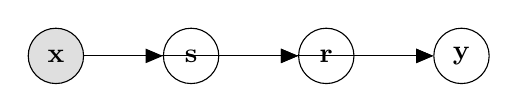
\begin{tikzpicture}
\node(x)[obs]{$\bx$};
\node(s)[latent, right =of x]{$\bs$};
\node(r)[latent, right =of s]{$\br$};
\node(y)[latent, right =of r]{$\by$};
\edge {x} {s};
\edge [bend right=30] {x} {r};
\edge {s} {r};
\edge [bend right=30] {s} {y};
\edge {r} {y};
\end{tikzpicture}
\label{tikz:simple}
\caption{}
\end{subfigure}

\begin{subfigure}[]{0.4\textwidth}
\centering
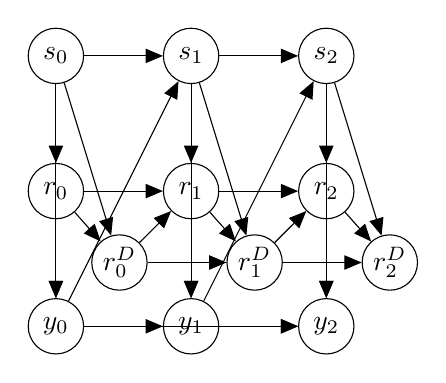
\begin{tikzpicture}
\node(s0)[latent]{$s_0$};
\node(r0)[latent, below =of s0]{$r_0$};
\node(r0d)[latent, below right =4mm and 3mm of r0]{$r_0^D$};
\node(y0)[latent, below =of r0]{$y_0$};
\node(s1)[latent, right =of s0]{$s_1$};
\node(r1)[latent, below =of s1]{$r_1$};
\node(r1d)[latent, below right =4mm and 3mm of r1]{$r_1^D$};
\node(y1)[latent, below =of r1]{$y_1$};
\node(s2)[latent, right =of s1]{$s_2$};
\node(r2)[latent, below =of s2]{$r_2$};
\node(r2d)[latent, below right =4mm and 3mm of r2]{$r_2^D$};
\node(y2)[latent, below =of r2]{$y_2$};

\edge {s0} {r0};
\edge [bend left=15] {s0} {r0d};
\edge [bend right=35] {s0} {y0};
\edge {r0} {y0};
\edge {r0} {r0d};

\edge {s1} {r1};
\edge [bend left=15] {s1} {r1d};
\edge [bend right=35] {s1} {y1};
\edge {r1} {y1};
\edge {r1} {r1d};

\edge {s2} {r2};
\edge [bend left=15] {s2} {r2d};
\edge [bend right=35] {s2} {y2};
\edge {r2} {y2};
\edge {r2} {r2d};

\edge {s0} {s1};
\edge {r0} {r1};
\edge {y0} {y1};
\edge {r0d} {r1};

\edge {r0d} {r1d};
\edge [bend left=15] {y0} {s1};

\edge {s1} {s2};
\edge {r1} {r2};
\edge [bend right=25] {y0} {y2};
\edge {y1} {y2};
\edge {r1d} {r2};

\edge {r1d} {r2d};
\edge [bend left=15] {y1} {s2};


\end{tikzpicture}
\label{tikz:full}
\caption{}
\end{subfigure}
\label{fig:pgm}
\caption{
(a) is a simplified graphical representation of the model
that ignores the temporal dependencies.
$\bx$ is the input data, $\bs$ the style, $\br$ the content,
and $\by$ the words of the summary.
(b) is the full graphical model.
We leave out conditioning on $\bx$ for brevity.
The new variables $r_i^D$ represent the duration a record is used.
}
\end{wrapfigure}
\paragraph{Argument for LVM}
\begin{enumerate}
\item The fully neural approach in \citep{puduppully2018contentselection} takes the output of
an information extraction system as the ground truth and trains a content planning model with
that assumption.
Any mistakes in the information extraction system will be replicated in the final model.
%In addition, the information extraction is trained via a heuristic alignment
%procedure that aligns words that appear in the database to records containing those words. 
%However, we argue that this particular procedure results in a compounding of mistakes.
% should use more precise notation here
Thus we argue that training the information extraction system by incorporating it
into an approximate posterior will improve performance as measured by
the likelihood of the data under our model.
\item As demonstrated in \citep{liang2009semalign},
a structured LVM results in qualitatively better segmentations than an unstructured one.
The latent variable formulation allows us to impose different inductive biases than a 
purely neural model.
For example, \citep{liang2009semalign} enforce monotonic alignments between text and records by using a 
hidden semi-markov model (HSMM).
\item Convincing templates from prior work \citep{wiseman2018template} indicate that the separation of
style and content is plausible.
\item Explicitly modeling characteristics such as the number of records in a given
sentence is possible in a latent variable model such as a HSMM.
\item Long-form text is HIGHLY multimodal, as there are many valid permutations of content. 
However, conditioning on content should help greatly with that multimodality.
\end{enumerate}

\paragraph{Approach and Methods}
% Proposal? Add more structure / modularity, principled inference...?
% Thesis: structure will help with controllability and LVM formulation
% with generalization as it presents a different inductive bias?
We would like to unify works from several directions:
\begin{enumerate}
\item Structure away content modeling through templates
\citep{sauper2009wiki,wiseman2018template}
\item Content planning and incorporating weak supervision
\citep{puduppully2018contentselection}
\item Efficient training methods for discrete LVMs \citep{deng2018vattn}
\end{enumerate}
% Elaborate on each of those points
We propose to model the conditional distribution of a summary given data as a 
hierarchical HSMM, as in \citep{liang2009semalign}.
Ignoring the temporal aspect of the model, we define a simplified model
with the following parts:
\begin{enumerate}
\item The given structured data $\bx$ 
\item Each sentence is generated using a style $s_i$
\item The content in each sentence $\br_i$ is chosen from $\bx$
after choosing a style $s_i$
\item The words in the summary $y_i$ are chosen conditioning on
the current content from $r_i$ as well as the style $c_i$
\end{enumerate}
We also present a more detailed model:
% Caveat: we don't want r_t to depend on r_{t-1} if starting a new sentence.
\begin{enumerate}
\item The style features $s_t\mid y_{t-1},s_{t-1},\bx\sim\Cat()$
\item The record choices $r_t\mid r_{t-1}^D,r_{t-1},s_t,\bx\sim\Cat()$
\item The record duration is given by 
$r_t^D\mid r_{t-1}^D=0,r_t\sim\Unif(1,\ldots,L)$
where $L$ is the max segment length and $r_t^D\mid r_{t-1}^D=x = x-1$

\item The words in the summary $y_t\mid y_{<t},r_t,s_t\sim\Cat()$
\end{enumerate}
See Figure~\ref{fig:pgm} for a simplified graphical depiction of the model.
We include a fully-specified slice of the time-series model as well,
but do not elaborate on it.

% too expensive to align to records since there may be many of them
As defined, the model would be very expensive to train via maximum marginal likelihood
training. We therefore propose to use the method proposed in \citep{deng2018vattn}
in order to make training tractable: namely define a variational approximation to the
posterior and use REINFORCE to maximize a lower bound on the marginal likelihood.
We also propose to incorporate intermediate weak supervision in the form of
heuristic record-to-text alignments.

% Should I explain why I propose a LVM versus a fully discriminative model?
% 
\paragraph{Intellectual Merit}
We hope to demonstrate the benefits of a hierarchical model in the task of text generation.
We propose a structure-aware content model similar to
work in \citep{sauper2009wiki,wiseman2017d2t,liang2009semalign}
that incorporates the computational advances in \citep{deng2018vattn}
in order to scale training.

\paragraph{Broader Impact}
The task of D2T itself is important, rather than simply a compromise between
short and long-form generation tasks.
Given a complicated set of structured data with possibly many records
which are irrelevant, an ideal D2T system would perform information triage by 
picking salient records then organize those records into prose.
This would be much easier to understand for someone unfamiliar with the
particular structure of the data and would aid in the dissemination of 
technological understanding.
With an interpretable LVM the user would also be able to examine the aligned
records that generated the summary, allowing the user to learn to read
the data by following the system's example.
% Stretch

\section{Outline}
\begin{enumerate}
\item Background
\begin{enumerate}
\item Breakdown of NLP into NLU and NLG
\item Importance of D2T, where we can learn a system to jointly perform NLU and NLG
\begin{enumerate}
\item Given the recent success with short-form generation in translation,
we can claim that we are good at generating text with strong conditioning.
In most cases, the source sentence provides all the information the model needs to translate.
However, for long-form translation current neural models do to not perform well.
%We hypothesize that this is because 
\item A compromise between short-form and long-form conditional generation  
\item Easily evaluable benchmark due to limited use of external knowledge
\item Convenient representation of input allows us to isolate progress
\item 
progress on generation metrics
\end{enumerate}
\item Introduce Rotowire \citep{wiseman2017d2t}
\begin{enumerate}
\item A summary of a basketball game is modelled conditioned on the box score
associated with that game.
\item The box score consists of a list of records associating an entity with a value.
Each record has a type which denotes the relationship between the entity and value
contained in the record,
for example: (type = POINTS, entity = Jeremy Lin, value = 19).
\end{enumerate}
\item Desiderata of Text Gen Systems, and how they are measured
\begin{enumerate}
\item Readability: How easy is it for a human to read the generated summary?
Refers to fluency and grammaticality, and is measured by BLEU as the two have been
shown to be correlated.
\item Informational Adequacy: How well does the model recreate the informational content
of a human-generated summary?
Measured through metrics concerning the selection and ordering of records.
% Discuss difficulties
\item Fidelity to conditioning: 
A lack of fidelity occurs if the model either ignores the data input and hallucinates
a value through the language model or if the model misaligns a record to a given segment of text.
\item Controllability:
Although a precise definition is available for dynamical systems,
we have yet to formalize a notion of controllability for NLG.
We loosely define controllability as the ability to apply constraints during inference.
% Maybe delta BLEU when using an oracle plan?
\end{enumerate}
\item Current trends addressing desiderata
\begin{enumerate}
\item Initially research focused largely on readability,
and improved BLEU scores through the use of conditional neural language models.
Compared to template-based methods, summaries were more fluent and natural.
However, by removing structure from the model and relying on the flexibility of neural networks
informational adequacy, fidelity, and controllability were sacrificed \citep{wiseman2017d2t}.
\item Subsequent work re-introduced the explicit modeling of content
\citep{puduppully2018contentselection}, which improved informational adequacy and
fidelity to conditioning through a latent content plan.
Although not entirely explored in the aforementioned work,
modeling the content plan also affords a degree of controllability.
By using oracle content plans extracted from the data,
they manage to obtain an upper bound on BLEU under their model.
\end{enumerate}
\end{enumerate}
\item Research Question
\begin{enumerate}
\item As research on D2T has embraced neural systems and end-to-end training
resulting in very unstructured models,
what is the benefit of imbuing more structure,
namely in the form of a hierarchical segmental model?
For the task of data-to-text, using a hierarchical HSMM allows us to model sentences
in a modular and controllable way;
we can control the number of records referred to in a sentence and the structure
of the sentence itself.
\end{enumerate}
\item Argument for a LVM:
Although the argument for modularity applies equally to models expressible as
neural networks as well as latent variable models, LVMs allow us to:
\begin{enumerate}
\item Learn an information extraction system jointly with the generative model.
\item Encode different inductive biases than neural models due to the ability to make hard decisions
and enforce structure.
\item Utilize indirect supervision over record alignments in a principled way.
\end{enumerate}
\item Approach and Methods
\begin{enumerate}
\item We propose a structure-aware content selection \citep{sauper2009wiki} model
as a hierarchical HSMM \citep{wiseman2018template}.
\item We incorporate weak supervision for the content planning model and
information extraction model through posterior constraints during sampling.
\item Our conditional generative model takes the form of a hierarchical
HSMM, where a sentence structure is first chosen, then the resulting records, and finally
the text to describe those records in accordance with the structure of the sentence.
\item At training time inference is quite difficult due to the large number of records,
so we resort to variational inference as in \citep{deng2018vattn}. 
\end{enumerate}
\item Extensions:
\begin{enumerate}
\item Fully generative model to reason about uncertainty over table values.
\item Fully generative model can include a model of table completion,
where unobserved values are functions of existing elements.
Maybe view this as a form of very limited reasoning.
\end{enumerate}
\item Relevance to BAA:
\begin{enumerate}
\item The thrust of information networks is concerned with representing
and acquiring knowledge graphs from various streams of data.
\item We propose to learn an information extraction system that is trained 
jointly with a generative model of the text.
\end{enumerate}
\end{enumerate}

\bibliographystyle{plainnat}
\bibliography{w}

\end{document}

